\documentclass[11pt]{article}

\usepackage{amsmath,amssymb}
\usepackage{float}
\usepackage[utf8]{inputenc}
\usepackage{hyperref}
\usepackage{graphicx}
\renewcommand{\baselinestretch}{1.1}

\title{Introduction to Word Embeddings (Part 2)}
\author{Aaron Geelon So}
\date{}

\begin{document}
\maketitle


In the previous \href{2017-07-24-word-embeddings-1.html}{post}, we
introduced what word embeddings are and what they can do. This time,
we'll try to make sense of them. What problem do they solve? How can
they help computers understand natural language?

\subsection*{Problem and Theory}\label{problem-and-theory}

See if you can guess what the word \emph{wapper} means from how it's
used in the following two sentences:

\begin{enumerate}
\def\labelenumi{\arabic{enumi}.}
\item
  After running the marathon, I could barely keep my legs from
  wappering.
\item
  Thou'll not see Stratfort to-night, sir, thy horse is wappered out.
  (Or perhaps a more modern take: I can't drive you to Stratford tonight
  for I'm wappered out).
\end{enumerate}

The second example is from the
\href{http://www.oed.com/view/Entry/225584}{Oxford English Dictionary}
entry. If you haven't guessed, the word was probably more popular in the
late-19th century. But it means \emph{to shake, especially from fatigue}
(and it might share the same linguistic roots as \emph{to waver}).

By now, you likely have a pretty good understanding of what \emph{to
wapper} means, if you like, even creating new sentences. Impressively,
you probably didn't need me to explicitly tell you the definition;
indeed, how many words in \emph{this} sentence did you learn by reading
a dictionary entry? We learn what words mean from their surrounding
\emph{contexts}.

This implies that even though it appears that the meaning of a word is
intrinsic to the word, \textbf{some of the meaning of a word also exists
in its context}.

Words, like notes on an instrument, do have their individual tones. But
it is their relationship with each other---their interplay---that gives
way to fuller music. Context enriches meaning.

So, take a context,
\[\textrm{After running the marathon, I could barely keep my legs from .}\]
We should have a sense of what words could fill the blank. Much more
likely to appear are words like \emph{shaking}, \emph{trembling}, and of
course, \emph{wappering}. Especially compared to nonsense like
\emph{pickled}, \emph{big data}, or even \emph{pickled big data}.

In short, the higher probability of appearing in this context
corresponds to greater shared meaning. From this, we can deduce the
\href{https://en.wikipedia.org/wiki/Distributional_semantics\#Distributional_hypothesis}{distributional
hypothesis}: words that share \emph{many} contexts tend to have similar
meaning.

What does this mean for a computer trying to understand words?

Well, if it can estimate how likely a word is to appear in different
contexts, then for most intents and purposes, the computer has learned
the meaning of the word.\footnote{And let's not get into any
  philosophical considerations of whether the computer really
  \emph{understands} the word. Come to think of it, how do I even know
  you understand a word of what I'm saying? Maybe it's just a matter of
  serendipity that the string of words I write make sense to you. But
  here I am really talking about how to oil paint clouds, and you think
  that I'm talking about machine learning.} Mathematically, we want to
approximate the probability distribution of
\[p(\textrm{ word } | \textrm{ context }) \quad\textrm{ or }\quad p(\textrm{ context }|\textrm{ word }).\]

Then, the next time the computer sees a specific context \(c\), it can
just figure out which words have the highest probability of appearing,
\(p(\textrm{ word }|\ c\ )\).

\subsubsection*{Challenges}\label{challenges}

The straightforward and naive approach to approximating the probability
distribution is:

\begin{itemize}
\item
  step 1: obtain a huge training corpus of texts,
\item
  step 2: calculate the probability of each \texttt{(word,context)} pair
  within the corpus.
\end{itemize}

The underlying (bad) assumption? The probability distribution learned
from the training corpus will approximate the theoretical distribution
over all word-context pairs.

However, if we think about it, the number of contexts is so great that
the computer will never see a vast majority of them. That is, many of
the probabilities \(p(\textrm{ word } |\ c\ )\) will be computed to be
0. This is mostly a terrible approximation.

The problem we've run into is the \textbf{curse of dimensionality}. The
number of possible contexts grows exponentially relative to the size of
our vocabulary---when we \emph{add} a new word to our vocabulary, we
more or less \emph{multiply} the number of contexts we can
make.\footnote{Consider a 20-word context. If we assume that the average
  English speaker's vocabulary is 25,000 words, then the increase of 1
  word corresponds to an increase of about \(7.2\times 10^{84}\)
  contexts, which is actually more than the
  \href{https://en.wikipedia.org/wiki/Observable_universe\#Matter_content}{number
  of atoms} in the universe. Of course, most of those contexts wouldn't
  make any sense.}

\begin{figure}[H]
\centering
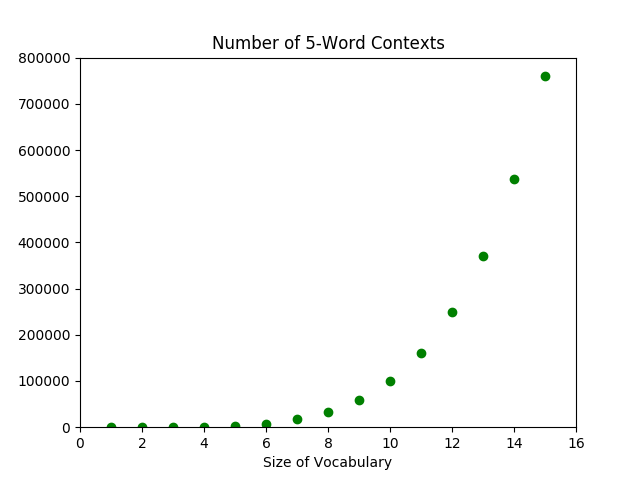
\includegraphics[width=300px]{files/curse.png}
\caption{The exponential growth of the number of contexts with
respect to the number of words.}
\end{figure}
We overcome the curse of dimensionality with \emph{word embeddings},
otherwise known as \textbf{distributed representations of words}.
Instead of focusing on words as individual entities to be trained
one-by-one, we focus on the attributes or \emph{features} that words
share.

For example, \emph{king} is a noun, singular and masculine. Of course,
many words are masculine singular nouns. But as we add more features, we
narrow down on the number of words satisfying each of those qualities.

Eventually, if we consider enough features, the collection of features a
word satisfies will be distinct from that of any other word.\footnote{The
  algorithm used by the Google researchers mentioned above assumes 300
  features.} This lets us uniquely represent words by their features. As
a result, we can now train features instead of individual
words.\footnote{The term \emph{distributed representation of words}
  comes from this: we can now represent words by their features, which
  are shared (i.e.~distributed) across all words. We can imagine the
  representation as a \emph{feature vector}. For example, it might have
  a `noun bit' that would be set to 1 for nouns and 0 for everything
  else. This is, however, a bit simplified. Features can take on a
  spectrum of values, in particular, any real value. So, feature vectors
  are actually vectors in a real vector space.}

This new type of algorithm would learn more along the lines of \emph{in
this context, nouns having such and such qualities are more likely to
appear} instead of \emph{we're more likely to see words X, Y, Z}. And
since many words are nouns, each context teaches the algorithm a little
bit about many words at once.

In summary, every word we train actually recalls a whole network of
other words. This allows us to overcome the exponential explosion of
word-context pairs by training an exponential number of them at a
time.\footnote{The distributed representations of words ``allows each
  training sentence to inform the model about an exponential number of
  semantically neighboring sentences,'' (Bengio 2003).}

\subsubsection*{A New Problem}\label{a-new-problem}

In theory, representing words by their features can help solve our
dimensionality problem. But, how do we implement it? Somehow, we need to
be able to turn every word into a unique \emph{feature vector}, like so:

\begin{figure}[H]
\centering
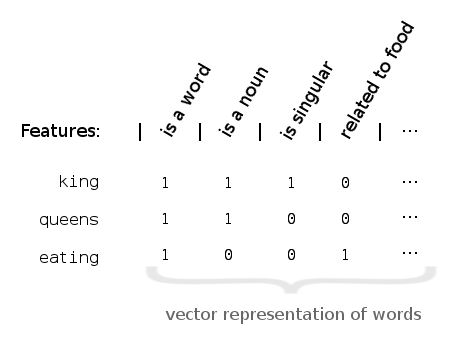
\includegraphics[width=300px]{files/vector.png}
The feature vector of the word \emph{king} would be
\(\langle 1, 1, 1,0,\dotsc\rangle\).
\end{figure}
But features like \emph{is a word} isn't very helpful; it doesn't
contribute to forming a \emph{unique} representation. One way to ensure
uniqueness is by looking at a whole lot of specific features. Take
\emph{is the word `king'} or \emph{is the word `gastroenteritis'}, for
example. That way, every word definitely corresponds to a different
feature vector:

\begin{figure}[H]
\centering
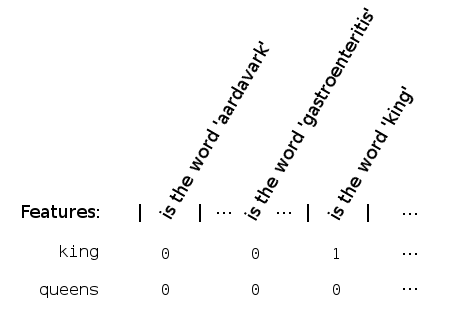
\includegraphics[width=300px]{files/vector2.png}
\caption{An inefficent representation defeating the purpose of
word embeddings.}
\end{figure}

This isn't a great representation though. Not only is this a very
inefficient way to represent words, but it also fails to solve the
original dimensionality problem. Although every word still technically
recalls a whole network of words, each network contains only one word!

Constructing the right collection of features is a hard problem. They
have to be not too general, not too specific. The resulting
representation of each word using those features should be unique. And,
we should limit the number of features to between 100-1000, usually.

Furthermore, even though it's simpler to think about binary features
that take on True/False values, we'll actually want to allow a spectrum
of feature values. In particular, any real value. So, feature vectors
are also actually vectors in a real vector space.

\subsubsection{A New Solution}\label{a-new-solution}

The solution to feature construction is: don't. At least not
directly.\footnote{This also means that there's probably not a `noun
  bit' in our representation, like in the figures above. There might not
  be any obvious meaning to each feature.}

Instead, let's revisit the probability distributions from before:
\[p(\textrm{ word }|\textrm{ context }) \quad\textrm{and}\quad p(\textrm{ context }|\textrm{ word }).\]
This time, words and contexts are represented by feature vectors:
\[\textrm{word}_i = \langle \theta_{i,1}, \theta_{i,2}, \dotsc, \theta_{i,300}\rangle,\]
which are just a collection of \emph{numbers}. This turns the
probability distributions from a functions over categorical objects
(i.e.~individual words) into a function over numerical variables
\(\theta_{ij}\). This is something that allows us to bring in a lot of
existing analytical tools---in particular, \emph{neural networks} and
other optimization methods.

The short version of the solution: from the above probability
distributions, we can calculate the probability of seeing our training
corpus, \(p(\textrm{corpus})\), which had better be relatively large. We
just need to find the values for each of the \(\theta_{ij}\)'s that
maximize \(p(\textrm{corpus})\).

These values for \(\theta_{ij}\) give precisely the feature
representations for each word, which in turn lets us calculate
\(p( \textrm{ word }|\textrm{ context })\).

Recall that this in theory teaches a computer the meaning of a word!

\subsubsection*{A Bit of Math}\label{a-bit-of-math}

In this section, I'll give enough details for the interested reader to
go on and understand the literature with a bit more ease.

Recall from previously, we have a collection of probability
distributions that are functions over some \(\theta_{ij}\)'s. The
literature refers to these \(\theta_{ij}\)'s as \emph{parameters} of the
probability distributions \(p(w|c)\) and \(p(c|w)\). The collection of
parameters \(\theta_{ij}\)'s is often denoted by a singular \(\theta\),
and the parametrized distributions by \(p(w|c;\theta)\) and
\(p(c|w;\theta)\).\footnote{The
  \href{https://en.wikipedia.org/wiki/Softmax_function}{softmax
  function} is often chosen as the ideal probability distribution. Let
  \(w_t\) be the vector representation of a word, and let \(C_t\) be the
  collection of words that have appeared in the context of \(w_t\).
  Then,
  \[p(w_c|w_t;\theta) = \frac{e^{w_c \cdot w_t}}{\sum_{w_{c'} \in C_t} e^{w_{c'} \cdot w_t}}.\]
  But other related functions are used in practice (for computational
  reason). The point here is that the parameters \(\theta\) are then
  optimized with respect to the selected distribution function.}

If the goal is to maximize the probability of the training corpus, let's
first write \(p(\textrm{corpus};\theta)\) in terms of \(p(c|w;\theta)\).

There are a few different approaches. But in the simplest, we think of a
training corpus as an ordered list of words, \(w_1, w_2, \dotsc, w_T\).
Each word in the corpus \(w_t\) has an associated context \(C_t\), which
is a collection of surrounding words.

\begin{align*}
\textrm{corpus: }\quad w_1\ | \ w_2\ | \ w_3\ | \quad \dotsm \quad & w _t \quad \dotsm \quad |\ w_{T-2} \ | \ w_{T-1} \ | \ w_T\\
& \,\Big\downarrow\\
\textrm{context of }w_t\textrm{: }\quad \big[ w_{t-n}\ \dotsm\ w_{t-1}\big]\ &w_t \ \big[w_{t+1}\ \dotsm\  w_{t+n} \big]
\end{align*}

\textbf{Diagram 1.} A corpus is just an ordered list of words. The
context \(C_t\) of \(w_t\) is a collection of words around it.\footnote{One
  can control the algorithm by specifying different hyperparameters: do
  we care about order of words? How many surrounding words do we
  consider? And on.}

For a given word \(w_t\) in the corpus, the probability of seeing
another word \(w_c\) in its context is \(p(w_c|w_t;\theta)\). Therefore,
the probability that a word sees all of the surrounding context words
\(w_c\) in the training corpus is
\[\prod_{w_c \in C_t} p(w_c|w_t;\theta).\] To get the total probability
of seeing our training corpus, we just take the product over all words
in the training corpus. Thus,
\[p(\textrm{corpus};\theta) = \prod_{w_t}\prod_{w_c \in C_t} p(w_c|w_t;\theta).\]

Now that we have the objective function,
\(f(\theta) = p(\textrm{corpus};\theta)\), it's just a matter of
choosing the parameters \(\theta\) that maximize \(f\).\footnote{This
  maximization problem is often equivalently written as
  \[\operatorname*{arg\,max}_\theta \sum_{w_t} \sum_{C_t} \log p(w_c|w_t;\theta).\]}
Depending on how the probability distribution is parametrized by
\(\theta\), this optimization problem can be solved using neural
networks. For this reason, this method is also called a
\href{https://en.wikipedia.org/wiki/Language_model\#Neural_language_models}{neural
language model} (NLM).

There are actually more layers of abstraction and bits of brilliance
between theory and implementation. While I hope that I've managed to
give you some understanding on where research is proceeding, the
successes of the current word embedding methods are still rather
mysterious. The intuition we've developed on the way is still, as
Goldberg, et. al. wrote, ``very hand-wavy'' (Goldberg 2014).

Still, perhaps this can help you have some intuition for what's going on
behind all the math when reading the literature. A lot more has been
written on this subject too; you can also take a look at the end of the
article where I list more
\protect\hyperlink{resources-ux5cux26-references}{resources} I found
useful.


\subsection*{Resources \& References}\label{resources-references}

I focused mainly on word2vec while researching neural language models.
However, do keep in mind that word2vec was just one of the earlier and
possibly more famous models. To understand the theory, I quite liked all
of the following. Approximately in order of increasing specificity,

\begin{itemize}
\item
  Radim Řehůřek's
  \href{https://rare-technologies.com/deep-learning-with-word2vec-and-gensim/}{introductory
  post} on word2vec. He also wrote and optimized the word2vec algorithm
  for Python, which he notes sometimes exceeds the performance of the
  original C code.
\item
  Chris McCormick's
  \href{http://mccormickml.com/2016/04/19/word2vec-tutorial-the-skip-gram-model/}{word2vec
  tutorial series}, which goes into much more depths on the actual
  word2vec algorithm. He writes very clearly, and he also provides a
  list of resources.
\item
  Goldberg and Levy 2014,
  \href{https://arxiv.org/abs/1402.3722}{word2vec Explained}, which
  helped me formulate my explanations above.
\item
  Sebastian Ruder's
  \href{http://ruder.io/word-embeddings-1/index.html}{word embedding
  series}. I found this series comprehensive but really accessible.
\item
  Bojanowski 2016, \href{https://arxiv.org/pdf/1607.04606.pdf}{Enriching
  word vectors with subword information}. This paper actually is for
  Facebook's fastText (which Mikolov is a part of), but it is based in
  part on word2vec. I found the explanation of word2vec's model in
  Section 3.1 transparent and concise.
\item
  Levy 2015,
  \href{https://levyomer.files.wordpress.com/2015/03/improving-distributional-similarity-tacl-2015.pdf}{Improving
  distributional similarity with lessons learned from word embeddings}
  points out that actually, the increased performance of word2vec over
  previous word embeddings models might be a result of ``hyperparameter
  optimizations,'' and not necessarily in the algorithm itself.
\end{itemize}

Listed here are the references I cited above.

{[}\href{http://www.jmlr.org/papers/volume3/bengio03a/bengio03a.pdf}{Bengio
2003}{]} Bengio, Yoshua, et al. ``A neural probabilistic language
model.'' Journal of machine learning research 3.Feb (2003): 1137-1155.

{[}\href{https://arxiv.org/pdf/1607.04606.pdf}{Bojanowski 2016}{]}
Bojanowski, Piotr, et al. ``Enriching word vectors with subword
information.'' arXiv preprint arXiv:1607.04606 (2016).

{[}\href{https://arxiv.org/pdf/1402.3722.pdf}{Goldberg 2014}{]}
Goldberg, Yoav, and Omer Levy. ``word2vec Explained: deriving Mikolov et
al.'s negative-sampling word-embedding method.'' arXiv preprint
arXiv:1402.3722 (2014).

{[}\href{http://www.deeplearningbook.org/}{Goodfellow 2016}{]}
Goodfellow, Ian, Yoshua Bengio, and Aaron Courville. Deep learning. MIT
press, 2016.

{[}\href{https://arxiv.org/pdf/1606.02820.pdf}{Hamilton 2016}{]}
Hamilton, William L., et al. ``Inducing domain-specific sentiment
lexicons from unlabeled corpora.'' arXiv preprint arXiv:1606.02820
(2016).

{[}\href{https://arxiv.org/pdf/1506.06726.pdf}{Kusner 2015}{]} Kusner,
Matt, et al. ``From word embeddings to document distances.''
International Conference on Machine Learning. 2015.

{[}\href{https://levyomer.files.wordpress.com/2015/03/improving-distributional-similarity-tacl-2015.pdf}{Levy
2015}{]} Levy, Omer, Yoav Goldberg, and Ido Dagan. ``Improving
distributional similarity with lessons learned from word embeddings.''
Transactions of the Association for Computational Linguistics 3 (2015):
211-225.

{[}\href{http://www.aclweb.org/anthology/N13-1090}{Mikolov 2013a}{]}
Mikolov, Tomas, Wen-tau Yih, and Geoffrey Zweig. ``Linguistic
regularities in continuous space word representations.'' hlt-Naacl. Vol.
13. 2013.

{[}\href{https://arxiv.org/pdf/1301.3781.pdf}{Mikolov 2013b}{]} Mikolov,
Tomas, et al. ``Efficient estimation of word representations in vector
space.'' arXiv preprint arXiv:1301.3781 (2013).

{[}\href{https://arxiv.org/pdf/1310.4546.pdf}{Mikolov 2013c}{]} Mikolov,
Tomas, et al. ``Distributed representations of words and phrases and
their compositionality.'' Advances in neural information processing
systems. 2013.

{[}\href{https://arxiv.org/pdf/1309.4168.pdf}{Mikolov 2013d}{]} Mikolov,
Tomas, Quoc V. Le, and Ilya Sutskever. ``Exploiting similarities among
languages for machine translation.'' arXiv preprint arXiv:1309.4168
(2013).

{[}\href{https://arxiv.org/pdf/1206.6426.pdf}{Mnih 2012}{]} Mnih,
Andriy, and Yee Whye Teh. ``A fast and simple algorithm for training
neural probabilistic language models.'' arXiv preprint arXiv:1206.6426
(2012).

{[}\href{https://arxiv.org/pdf/1411.2738.pdf}{Rong 2014}{]} Rong, Xin.
``word2vec parameter learning explained.'' arXiv preprint
arXiv:1411.2738 (2014).
\end{document}
